\chapter{Unit Step and Unit Impulse Functions (Oppenheim 1.4-1.5)}

\section{Discrete Time}
\begin{definition}
    [Discrete Unit Impulse Function]
    The \textbf{discrete unit step function} $u[n]$ is defined as
    $$ \delta[n] = \begin{cases}
            1 & n = 0            \\
            0 & \forall n \neq 0
        \end{cases} $$
\end{definition}


\begin{corollary}
    [Multiplication by Unit Impulse Function]
    Let $x[n]$ be a discrete-time signal. Then, the multiplication of $x[n]$ by the unit step function $u[n]$ is given by
    $$ x[n]\delta[n - k] = x[k] $$
\end{corollary}

\begin{definition}
    [Discrete Unit Step Function]
    The \textbf{discrete unit step function} $u[n]$ is defined as
    $$ u[n] = \begin{cases}
            1 & n \geq 0 \\
            0 & n < 0
        \end{cases} $$
\end{definition}
\begin{corollary}
    [First Order Difference of Unit Step Function]
    The first order difference of the unit step function is given by
    $$ u[n] - u[n - 1] = \delta[n] $$
\end{corollary}

\begin{remark}
    \textbf{First order differences} in discrete-time signals are equivalent to \textbf{derivatives} in continuous-time signals.
\end{remark}

\begin{corollary}
    [Running Sum of the Delta Function]
    The running sum of the delta function is given by
    $$ \sum_{m = -\infty}^{n} \delta[m] = u[n] $$
\end{corollary}

\begin{remark}
    \textbf{The running sum} of in discrete time is equivalent to the \textbf{integral} in continuous time.
\end{remark}

\section{Continuous Time}
\begin{definition}
    [Unit step function]
    The \textbf{unit step function} $u(t)$ is defined as
    $$ u(t) = \begin{cases}
            1 & t \geq 0 \\
            0 & t < 0
        \end{cases} $$
\end{definition}

\begin{definition}
    [Unit impulse function]
    The \textbf{unit impulse function} $\delta(t)$ is defined as the integral over all time of the unit step function
    $$ \delta(t) = \int_{-\infty}^{\infty} \delta(t) d$$
    But
\end{definition}

\begin{remark}
    The unit impulse function is a \textbf{distribution} and not a function, and the derivative \textbf{dos not exist} at $t = 0$.
\end{remark}

\begin{corollary}
    [Derivative of the Unit Step Function]
    \begin{align*}
        \delta_{\Delta} (t) = \frac{d}{dt} u_{\Delta}(t) \quad \text{as } \Delta \to 0
    \end{align*}
\end{corollary}

% \begin{figure}
%     \centering
%     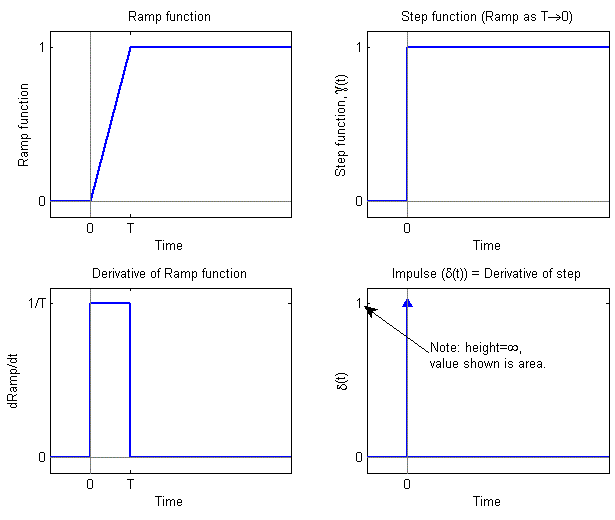
\includegraphics[width=0.5\textwidth]{LECTURE_7/impulse.png]}
%     \caption{Unit Impulse Function}
%     \label{fig:impulse}
% \end{figure}


\begin{theorem}
    [Multiplication by Unit Impulse Function]
    Let $x(t)$ bea signal and consider the procuct of $x(t)$ with the unit impulse function $\delta_{\Delta}(t)$.
    $$ \lim_{\Delta \to 0} x(t) \delta_{\Delta}(t - t_0) = x(t_0) $$
\end{theorem}